\documentclass[10pt]{article}
\usepackage{helvet}
\renewcommand{\familydefault}{\sfdefault}

\usepackage{graphicx}
\usepackage[english]{babel}


\usepackage{tikz}
\usetikzlibrary{matrix, fit, positioning, calc, shapes.arrows}
\usepackage[absolute,overlay]{textpos}
\usepackage{tabularx}
\usepackage{colortbl}
\setlength{\tabcolsep}{3pt}
\usepackage{gensymb}
\usepackage[breakall]{truncate}

\newcommand{\grid}{
  \draw[step=.5cm,draw opacity=.5] (0,0) grid (\the\paperwidth,\the\paperheight);
  \foreach \x in {1,2,...,20}
    \draw[text=black] (\x,.15) node {\footnotesize \x};
  \foreach \y in {1,2,...,27}
    \draw[text=black] (.2,\y) node {\footnotesize \y};
}
\newcommand{\nogrid}{
  \draw[step=.5cm,draw opacity=0] (0,0) grid (\the\paperwidth,\the\paperheight);
}

% Define colors for map scale
\definecolor{green}{HTML}{00B04F}
\definecolor{yellow}{HTML}{FFFF00}
\definecolor{orange}{HTML}{FF9900}
\definecolor{red}{HTML}{FF0000}

%Define colors for tags
\definecolor{greentag}{HTML}{73B688}
\definecolor{yellowtag}{HTML}{F5F56C}
\definecolor{redtag}{HTML}{FF5252}

%-------------------------------------------------------------------------------
% Begin document
%-------------------------------------------------------------------------------
\begin{document}
\thispagestyle{empty}

% Styles
\tikzset{
  % Arrow for Hazus losses
  loss arrow/.style={
    draw,
    thick,
    shape=single arrow,
    minimum height=1.7cm,
    shape border rotate=90,
  },
  % Font for text outside of tables
  ntext/.style={
    font=\small,
    inner sep=0pt,
    outer sep=0pt
  },
  % Font for disclaimers
  ftext/.style={
    font=\footnotesize,
    inner sep=0pt,
    outer sep=0pt
  },
  % h1 style
  h1/.style={
    align=center,
    text depth=0.6ex,
    text height=1.6ex,
    inner sep=0pt,
    outer sep=0pt,
    font=\bf\Large
  },
  % h2 style
  h2/.style={
    align=center,
    inner sep=0pt,
    outer sep=0pt,
    font=\bf\large,
    anchor=center,
    text height=1.5ex,
    text depth=0.5ex
  },
  % Styles for color bar
  cbar/.style={font=\bf\footnotesize,rectangle,draw,minimum width=3.2465cm,
    anchor=west,inner sep=0pt,outer sep=0pt,text height=1.6ex,
    text depth=0.5ex
    },
  % Style for footnotes
  fn/.style={
    font=\scriptsize,
    inner xsep=0,
    inner ysep=1pt,
    text height=1.3ex,
    text depth=0.2ex
  },
  % Style for small info stuff in title bar
  info/.style={
    font=\footnotesize,
    inner xsep=0,
    inner ysep=1pt,
    text height=1.3ex,
    text depth=0.2ex
  },
  % For placing a node between two other nodes
  between/.style args={#1 and #2}{
    at = ($(#1)!0.5!(#2)$)
  }
}

% Setup axes
\begin{textblock}{1}(0,0)
% Start tikz
\begin{tikzpicture}
% Turn grid on or off
\nogrid

%----------------------------------
% PAGER Content First
%----------------------------------

%-------------------------------------------------------------------------------
% Alerts and histograms with estimated fatalities and losses 
%-------------------------------------------------------------------------------

% Outline
\node[draw,thick,minimum width=20.3cm,minimum height=4.2cm](abox) at (10.3cm,22.5cm){};

% Histogram - fatalities
\node[above=0 of abox.south west,anchor=south west,
  xshift=2pt,yshift=2pt,inner sep=0,outer sep=0](fhist){
\includegraphics[width=6.75cm,trim={1.8cm 1.3cm 1.3cm -1.25cm},clip]
  {[VERSIONFOLDER]/alertfatal.pdf}
};
\node[h1,xshift=1mm,below=1.7mm of abox.north west,
      anchor=north west]{
  PAGER Estimated Fatalities
};

% Histogram - economic
\node[above=0 of abox.south east,anchor=south east,
  xshift=-2pt,yshift=2pt,inner sep=0,outer sep=0](ehist){
\includegraphics[width=6.75cm,trim={1.8cm 1.3cm 1.3cm -1.25cm},clip]
  {[VERSIONFOLDER]/alertecon.pdf}
};
\node[h1,xshift=0.7mm,below=1.7mm of abox.north east,
      anchor=north east]{
  PAGER Est Economic Losses
};

% PAGER summary statement
\node[ntext,xshift=-1.5mm,below=1.5mm of abox.north,anchor=north,
  text width=6cm,align=justify](impact1){
  [IMPACT1]
};
\node[ntext,below=1.5ex of impact1.south,anchor=north,
  text width=6cm,align=justify](impact2){
  [IMPACT2]
};

% Summary level
\node[circle,draw,fill=[ALERTFILL],minimum size=12mm]
  (scir) 
  at (10.5cm,26.75cm) {};

\node[h2,left=1mm of scir.west,anchor=east,text width=2.5cm,
      align=right,yshift=10pt]{
  Earthquake \\ Shaking
};

\node[h2,right=1mm of scir.east,anchor=west,text width=2.5cm,
      align=left,yshift=10pt]{
  [SUMMARYCOLOR] \\ Alert
};

%-------------------------------------------------------------------------------
% Header stuff
%-------------------------------------------------------------------------------

% Tsunami
\node[info,above=1pt of abox.north west,anchor=south west](tsunami){
  \color{red}\textbf{[TSUNAMI]}
};

% Location
\node[info,above=-1pt of tsunami.north west,anchor=south west](loc){
  Location: [LAT]\degree\,[HEMILAT] [LON]\degree\,[HEMILON] Depth: [DEPTH] km
};

% Origin time
\node[info,above=0 of loc.north west,anchor=south west,
  inner ysep=0](otime){
  Origin Time: [ORIGTIME] UTC ([LOCALTIME] local)
};

% Mag and location
\node[h1,above=0 of otime.north west,anchor=south west,
  inner ysep=0](magloc){
  [MAGLOC]
};

% Elapsed time
\node[info,above=1pt of abox.north east,anchor=south east](elapsed){
  [ELAPSED]};

% Version
\node[h1,above=2pt of elapsed.north east,anchor=south east,
      inner sep=0,outer sep=0](version){[VERSION]};
\node[h1,above=5pt of version.north east,anchor=south east,
      inner sep=0,outer sep=0,yshift=0pt](pager){Hazus-PAGER};

% Logos
\node[above=0cm of pager.north east,anchor=south east,
      inner sep=0,outer sep=0,yshift=1mm](fema){
  \includegraphics[scale=0.32]{[HOMEDIR]/losspager/logos/FEMA_logo.pdf}
};
\node[above=2pt of magloc.north west,anchor=south west,
      inner sep=0,outer sep=0,yshift=2mm](usgs){
  \includegraphics[scale=0.17]{[HOMEDIR]/losspager/logos/USGSid.pdf}
};

%----------------------------------
% Hazus Content Second
%----------------------------------

%-------------------------------------------------------------------------------
% Rectangle around Hazus info
%-------------------------------------------------------------------------------
\node[below=0.2cm of abox.south,draw,thick,minimum width=20.3cm,minimum height=18.6cm](hazbox){};

%-------------------------------------------------------------------------------
% Hazus loss estimate arrow and pass through box
%-------------------------------------------------------------------------------
\node[rectangle,fill=white,left=[BOXSHIFT]cm of hazbox.north east,anchor=north west,minimum width=1.85cm, minimum height=0.4cm,yshift=1.6mm]{}; 
\node[loss arrow,left=[ARROWSHIFT]cm of hazbox.north east,fill=[HAZUS_SUMMARY]](hazarrow) {};
\node[h2,left=3.6mm of hazarrow.east,anchor=east,text width=2.5cm,
      align=right,yshift=-3pt]{
  Hazus \\ Estimate
  };

%-------------------------------------------------------------------------------
% Tagging estimates
%-------------------------------------------------------------------------------
\node[h1,xshift=1mm,below=2mm of hazbox.north west,
      anchor=north west]{
  Hazus Building Tagging Estimates
};

%Green Tag
\node[xshift=0.3cm,below=0.6cm of hazbox.north west,anchor=north west]{
 
\includegraphics[width=3.8cm,height=4cm]
    {[HOMEDIR]/losspager/logos/green_tag.pdf}
};      
\node[ntext,xshift=0.45cm,below=0.8cm of hazbox.north west,anchor=north west,
   text width=3.4cm](gtag){
   [GREEN_TAG_TABLE]
};

%Yellow Tag
\node[xshift=4.45cm,below=0.6cm of hazbox.north west,anchor=north west]{
 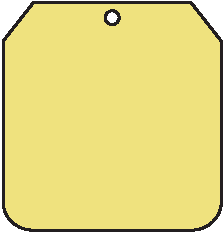
\includegraphics[width=3.8cm,height=4cm]
    {[HOMEDIR]/losspager/logos/yellow_tag.pdf}
};      
\node[ntext,xshift=4.62cm,below=0.8cm of hazbox.north west,anchor=north west,
   text width=3.4cm](ytag){
   [YELLOW_TAG_TABLE]
};

%Red Tag
\node[xshift=8.6cm,below=0.6cm of hazbox.north west,anchor=north west]{

\includegraphics[width=3.8cm,height=4cm]
    {[HOMEDIR]/losspager/logos/red_tag.pdf}
};      
\node[ntext,xshift=8.79cm,below=0.8cm of hazbox.north west,anchor=north west,
   text width=3.4cm](rtag){
   [RED_TAG_TABLE]
};

%-------------------------------------------------------------------------------
% Losses by census tract map
%-------------------------------------------------------------------------------

% Add map
\node[draw,thick,rectangle,inner sep=-0.5pt,outer sep=0,
      xshift=0.3mm,above=0.2pt of hazbox.south west,anchor=south west](cmap){
  \includegraphics[width=13cm]
    {[VERSIONFOLDER]/hazus_map.png}
};

% Then draw loss scale
\node[cbar,fill=green,xshift=-0.3pt,above=-0.3pt of cmap.north west,anchor=south west](gdel) {\textless\textdollar1M};
\node[cbar,fill=yellow,right=0 of gdel](ydel) {\textdollar1M - \textdollar100M};
\node[cbar,fill=orange,right=0 of ydel](odel) {\textdollar100M - \textdollar1B};
\node[cbar,fill=red,right=0 of odel](rdel){\textdollar1B+};
\node[rectangle,inner xsep=0,xshift=1mm,above=4mm of cmap.north west,anchor=south west,h1]
     (poptitle){Estimated Direct Economic Loss by Census Tract};

%-------------------------------------------------------------------------------
% Map side bar
%-------------------------------------------------------------------------------

% Width of side bar
\def \barwidth{7.1cm}

% Top block: Direct Economic Losses by County
\node[h2,below=1.33cm of hazbox.north east,anchor=north east,
  yshift=0mm] (del){
  Direct Economic Losses by County
};
\node[ntext,below=0.9pt of del.south west,anchor=north west,
  text width=\barwidth,align=justify](deltab){
  [DEL_TABLE]
  };

% Second block: Non-Fatal Injuries by County
\node[h2,below=5.65cm of hazbox.north east,anchor=north east,
  text width=\barwidth]
     (nfi){
  Non-Fatal Injuries by County
};
\node[ntext,below=0.9pt of nfi.south west,anchor=north west,
  text width=\barwidth]
     (nfitab){
  [NFI_TABLE]
};

% Third block: Shelter Needs by County
\node[h2,below=10cm of hazbox.north east,anchor=north east,
  text width=\barwidth]
     (shelter){
  Shelter Needs by County
};
\node[ntext,below=0.9pt of shelter.south west,anchor=north west,
  text width=\barwidth]
     (sheltertab){
  [SHELTER_TABLE]
};

% Bottom block: Earthquake Debris
\node[h2,below=15.1cm of hazbox.north east,anchor=north east,
  text width=\barwidth]
     (debris){
  Earthquake Debris
};
\node[ntext,below=0.9pt of debris.south west,anchor=north west,
  text width=\barwidth]
     (debristab){
  [DEBRIS_TABLE]
};

%-------------------------------------------------------------------------------
% Footers
%-------------------------------------------------------------------------------
\node[info,below=0 of hazbox.south west,anchor=north west](mapfn1){
  Hazus-PAGER content is automatically generated. Limitations of input data may add uncertainty.
};
\node[ftext,font=\bf\footnotesize,below=1pt of mapfn1.south west,anchor=north west](eventurl){
  [EVENTURL]
};
\node[ftext,font=\bf\footnotesize,below=1pt of eventurl.south west,anchor=north west](hazusurl){
  [HAZUSURL]
};
\node[ftext,font=\bf\footnotesize,below=2pt of hazbox.south east,anchor=north east](eventid){
  [EVENTID]
};

\end{tikzpicture}
\end{textblock}

\end{document}
